\chapter*{2 Versuchsdurchführung und Auswertung}
\addcontentsline{toc}{chapter}{2 Versuchsdurchführung und Auswertung}
\setcounter{chapter}{2}
\setcounter{section}{0}
\setcounter{subsection}{0}
 
    \section{Versuch 1 - Bestimmung der Viskosität von Getriebeöl mit der Kugelfallmethode}
    \label{sec:Versuch1}
        
        \subsection{Aufbau \& Durchführung}

            In Versuch 1 wird die dynamische Viskosität von Getriebeöl mit Hilfe der Kugelfallmethode bestimmt. Der Versuchsaufbau sieht wie folgt aus:
            Ein Glaszylinder, welcher mind. $30\ \mathrm{cm}$ hoch ist, wird mit Getriebeöl OKS 3740 befüllt. Nun wird eine Fallstrecke $L$ von $15\ \mathrm{cm}$ markiert. Diese hat mind. $5\ \mathrm{cm}$ Abstand zur Öffnung des Gefäßes. Anschließend werden jeweils 10 Kugeln in der Mitte des Gefäßes fallen gelassen und die Fallzeit im Abschnitt $L$ gemessen. Dies wird für die Kugeldurchmesser $d = 1, 2, 3\ \mathrm{mm}$ und $4\ \mathrm{mm}$ wiederholt. Die $3\ \mathrm{mm}$-Kugel wird 30 Mal gemessen und später eine Verteilung zufällig schwankender Messwerte graphisch darzustellen.
            Die Viskosität lässt sich dann über die Formel der dynamischen Viskosität $\eta$ berechnen, oder mit Hilfe eines Graphens.

        \subsection{Auswertung}

            Zunächst wurde der Durchmesser $d$ stichprobenartig von $3$ Kugeln gemessen:

            \begin{table}[H]
                \centering
                \begin{tabular}{|l||r||r|r|r|}
                    \hline
                    & $d_{1}$ & $d_{2}$ & $d_{3}$ & $d_{4}$\\
                    \hline \hline
                    Mittelwert $[\mathrm{mm}]$ & $0.993$ & $1.997$ & $2.99$ & $3.99$\\
                    Standartabweichung $[\mathrm{mm}]$ & $0.00577$ & $0.00577$ & $0.00000$ & $0.00577$\\
                    \hline
                \end{tabular}
                \caption{Ergebnis der Messung der Kugeldurchmesser.}
                \label{tab:MesswerteDurchmesser}
            \end{table}

            Danach wurden die Fallzeiten $t_{i}$ der Kugeln gemessen:

            \begin{table}[H]
                \centering
                \begin{tabular}{|l||r|r|r|r|}
                    \hline
                    $n$ & $t_{1}$ & $t_{2}$ & $t_{3}$ & $t_{4}$\\
                    \hline \hline
                    1 & 79,23    & 20,17    & 9,28    & 5,28\\
                    2 & 79,47    & 20,47    & 9,25    & 5,31\\
                    3 & 79,88    & 20,22    & 9,14    & 5,38\\
                    4 & 79,07    & 20,49    & 9,25    & 5,39\\
                    5 & 79,66    & 20,58    & 9,28    & 5,31\\
                    6 & 79,07    & 20,06    & 9,25    & 5,43\\
                    7 & 79,35    & 20,11    & 9,08    & 5,41\\
                    8 & 78,42    & 20,21    & 9,28    & 5,41\\
                    9 & 76,95    & 20,19    & 9,29    & 5,23\\
                    10 & 79,36   & 19,60    & 9,34    & 5,40\\
                    11 &         &          & 9,27    &     \\
                    12 &         &          & 9,10    &     \\
                    13 &         &          & 9,24    &     \\
                    14 &         &          & 9,25    &     \\
                    15 &         &          & 9,17    &     \\
                    16 &         &          & 9,26    &     \\
                    17 &         &          & 9,14    &     \\
                    18 &         &          & 9,30    &     \\
                    19 &         &          & 9,19    &     \\
                    20 &         &          & 9,29    &     \\
                    21 &         &          & 9,79    &     \\
                    22 &         &          & 9,20    &     \\
                    23 &         &          & 9,16    &     \\
                    24 &         &          & 9,19    &     \\
                    25 &         &          & 9,01    &     \\
                    26 &         &          & 9,10    &     \\
                    27 &         &          & 9,22    &     \\
                    28 &         &          & 9,20    &     \\
                    29 &         &          & 9,05    &     \\
                    30 &         &          & 9,14    &     \\
                    \hline
                    Mittelwert $[s]$ & 79,00 & 20,20 & 9,20 & 5,36\\
                    Standardabweichung $[s]$ & 0,83423 & 0,27681 & 0,13433 & 0,06737\\
                    Mittelwert der Standardabweichung $[s]$ & 0,26381 & 0,08753 & 0,02453 & 0,02130\\
                    \hline
                \end{tabular}
                \caption{Ergebnis der Messung der Fallzeiten.}
                \label{tab:MesswerteFallzeiten}
            \end{table}

            Die Länge $L$ der Fallstrecke beträgt $15\ \mathrm{cm}$. Die Dichte der Kugeln (V2A-Stahl) $\rho_{\mathrm{K}}$ und die Dichte des Getriebeöls OKS 3740 $\rho_{\mathrm{F}}$ betragen:

            \begin{align}
                \rho_{\mathrm{K}} &= 7900\ \mathrm{\frac{kg}{m^{3}}}\\
                \rho_{\mathrm{F}} &= 850\ \mathrm{\frac{kg}{m^{3}}}
            \end{align}

            Somit lassen sich mit der Formel für die dynamische Viskosität $\eta$:

            \begin{equation}
                \eta = \frac{(\rho_{\mathrm{K}} - \rho_{\mathrm{F}}) \cdot g}{18 \cdot L} \cdot d^{2} \cdot t
            \end{equation}

            die Viskosität $\eta$ der Flüssigkeit berechnen. Die Fallbeschleunigung $g$ beträgt $9,81\ \mathrm{\frac{m}{s^{2}}}$.

            Für die Größtfehlerabschätzung werden folgende Werte verwendet:

            \begin{table}[H]
                \centering
                \begin{tabular}{|l||r|}
                    \hline
                    $\Delta L [\mathrm{mm}]$ & 5.00\\
                    \hline
                    $\Delta d [\mathrm{mm}]$ & 0.01\\
                    \hline
                    $\Delta t [\mathrm{s}]$ & 0.4\\
                    \hline
                \end{tabular}
                \caption{Fehlerabschätzung der Messwerte.}
                \label{tab:Fehlerabschaetzung}
            \end{table}

            Der Wert $0.4$ ergibt sich aus der zweifachen Reaktionszeit des Menschen.

            Mit diesen Werten lässt sich nun das folgende Ergebnis berechnen:

            \begin{table}[H]
                \centering
                \begin{tabular}{|l||r|r|r|r|}
                    \hline
                    & $d_{1}$ & $d_{2}$ & $d_{3}$ & $d_{4}$\\
                    \hline \hline
                    Viskosität $[\mathrm{Pa \cdot s}]$ & $1.99502$ & $2.06089$ & $2.10923$ & $2.18428$\\
                    \hline
                    $\frac{\Delta L}{L}$ & $0.03333$ & $0.03333$ & $0.03333$ & $0.03333$\\
                    $\frac{\Delta d}{d}$ & $0.02013$ & $0.01002$ & $0.00669$ & $0.00501$\\
                    $\frac{\Delta t}{t}$ & $0.00506$ & $0.01979$ & $0.04337$ & $0.07470$\\
                    \hline
                    Größtfehler $[\mathrm{Pa \cdot s}]$ & $0.11676$ & $0.13013$ & $0.17589$ & $0.24691$\\
                    \hline
                \end{tabular}
            \end{table}

            Der Mittelwert der Viskosität beträgt somit: $\eta = 2.08736\ \mathrm{Pa \cdot s}$.

            Trägt man die Mittelwerte der Fallzeiten über $\frac{1}{d^{2}}$ in einem Graphen (\ref{fig:graph_01}) auf und lässt sich die Steigung berechnen, so erhält man eine zweite Möglichkeit die Viskosität zu berechnen. Die Steigung $m$ der Gerade entspricht in unserem Fall dem Wert: $78.219$. Die Viskosität $\eta$ lässt sich dann mit der Formel: 

            \begin{equation}
                \eta = \frac{m \cdot (\rho_{\mathrm{K}} - \rho_{\mathrm{F}}) \cdot g}{18 \cdot L}
            \end{equation}

            bestimmen. Das Ergebnis lautet: $\eta = 2.00074\ \mathrm{Pa \cdot s}$.

            \begin{figure}
                \centering
                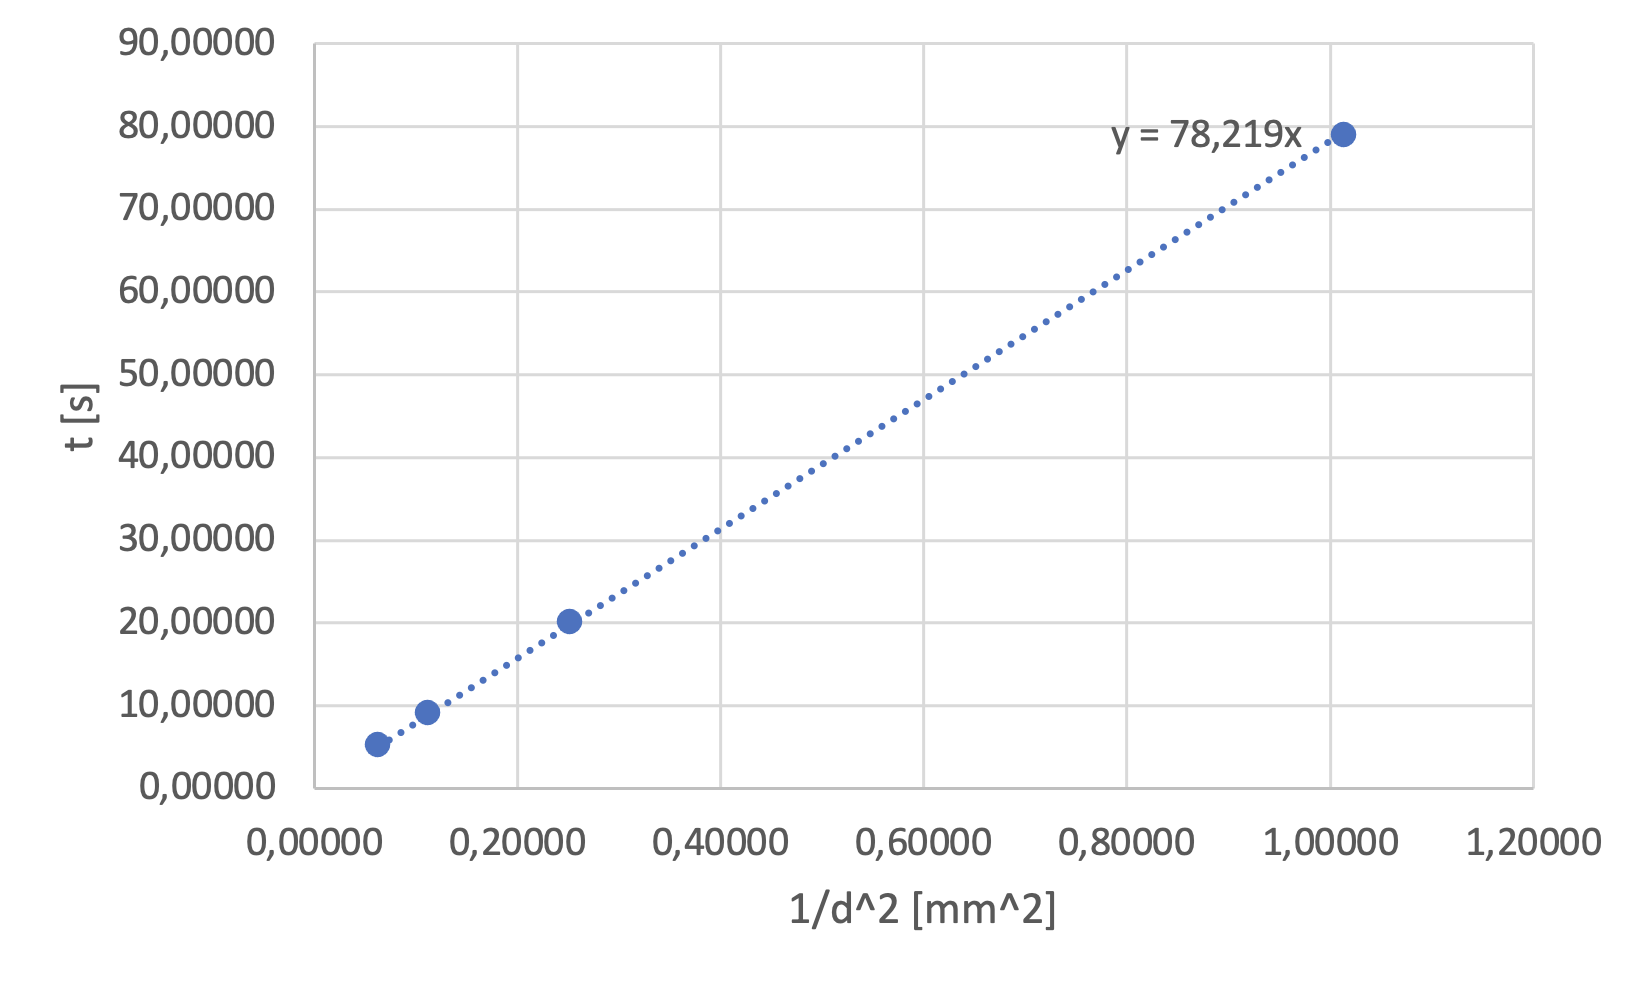
\includegraphics[width=0.8\textwidth]{bilder/Diagram_01.png}
                \caption{Fallzeiten über $\frac{1}{d^{2}}$.}
                \label{fig:graph_01}
            \end{figure}
        
        \subsection{Diskussion}

            \textcolor{red}{TODO}

            Notizen:
            Warum ist zweiter Viskosität Wert niedriger $\rightarrow$ wegen $1/d^2$, gewichtung liegt auf 1mm kugel, die genauer ist, da mehr laminare strömung und weniger turbulenz
            Warum generll höher $\rightarrow$ luftemperatur 20 Grad, aber flüssigkeit vielleicht nicht, allgmeine Messfehler
        
    \section{Versuch 2 - Bestimmung der Glycerinkonzentration mit dem Kapillarviskosimeter}
    \label{sec:Versuch2}

        \subsection{Aufbau \& Durchführung}
            
            In Versuch 2 wird die kinematische Viskosität $\nu$ einer Glycerin-Wasser-Mischung mit Hilfe eines Kapillarviskosimeters bestimmt. Der Versuchsaufbau sieht wie folgt aus.

            \begin{figure}[h]
                \centering
                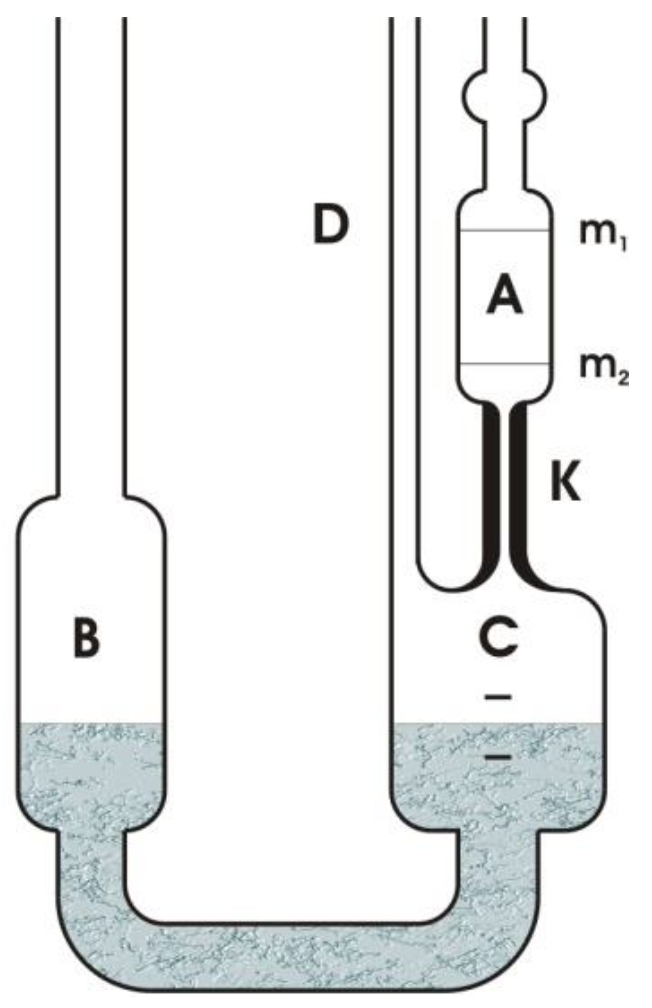
\includegraphics[width=0.5\textwidth]{bilder/Kapillarviskosimeter.png}
                \caption{Aufbau des Kapillarviskosimeters.}
                \label{fig:Kapillarviskosimeter}
            \end{figure}

            Ein Wassertank ist mit Wasser befüllt und wird auf konstante $30\ \mathrm{^\circ C}$ erwärmt. In diesen Wassertank wird das Kapillarviskosimeter eingetaucht. Ein genauerer Aufbau des Kapillarviskosimeters ist in Abbildung \ref{fig:Kapillarviskosimeter} zu sehen. Dieses Funktioniert so, dass die Öffnung D zugehalten wird, die Flüssigkeit durch Ansaugen an Öffnung A, nach oben gesaugt wird, bis die Flüssigkeit den Raum A komplett ausfüllt, sodass die Flüssigkeit zwischen $m_1$ und $m_2$ vorhanden ist. Danach wird die Öffnung an D geöffnet und auch an A. Dann wird die Zeit gemssen, die die Flüssigkeit benötigt um die Strecke zwischen $m_{1}$ und $m_{2}$ abzusinken. Mit den Messwerten und der Formel

            \begin{equation}
                \nu = K \cdot t
            \end{equation}

            lässt sich die kinematische Viskosität berechnen. Dabei ist $K$ eine Konstante, die für jedes Kapillarviskosimeter unterschiedlich ist. Diese Werte sind allerdings schon vorgegeben.

        \subsection{Auswertung}

        \subsection{Diskussion}